%%%%%%%%%%%%%%%%%%%%%%%%%%%%
% Master's Thesis          %	    										
% Fabian Burth, 2022-08-01 %
%%%%%%%%%%%%%%%%%%%%%%%%%%%%

\npchapter{Foundations}
\section{Terminology}
This section explains several abbreviations and standards which are commonly mentioned alongside the topics \textit{Software Bill of Materials}, \textit{Vulnerability Management} and \textit{Open Source Licensing} and are thus essential for the further understanding.\\

\noindent
\textbf{Common Platform Enumeration (CPE)}: The CPE specification originally created by MITRE and now maintained by NIST provides a naming scheme for IT assets such as software. It may be used to uniquely determine a specific software and its version. This way a CPE enables cross referencing to other sources of information. The commonly used CPE naming scheme is structured as follows:\\
\noindent
\begin{lstlisting}[caption=CPE Formatted String Binding, captionpos=b, label=lst:CPE]
cpe:2.3: part : vendor : product : version : update : edition : language : sw_edition : target_sw : taget_hw : other
\end{lstlisting}

\noindent
Thereby \lstinline|part| may be \textit{a} for applications, \textit{o} for operating systems, and \textit{h} for hardware devices. \lstinline|edition| is a legacy attribute in the current version of the specification and may be omitted where not required for backward compatibility. The attributes after \lstinline|edition| were newly introduced in this version and are referred to as \textit{extended attributes}. \lstinline|sw_edition| should characterize a particular market or class of users a product is tailored to (e.g. online), \lstinline|target_sw| a software computing environment (e.g. linux), \lstinline|target_hw| the instruction set architecture (e.g. x86), and \lstinline|language| the language supported in the user interface \cite{CPESpec}.\\

Package Information:
	Maven Coordinates (GAV - groupId:artifactId:version)
	NPM Coordinates 
	Package URLs
CPE (Common Platform Enumeration):
CVE (Common Vulnerabilities and Exposures):
CNA (CVE Numbering Authorities):
CWE (Common Weakness Enumeration):
CVSS (Common Vulnerability Scoring System):
NVD (U.S. National Vulnerability Database):
CERT/CC Vulnerability Notes Database: 
Vulnerability:
Exposure:

\section{Software Bill of Materials}
A \textit{Software Bill of Materials} is an inventory of the components used in a software. It ideally contains all direct and transitive components and their dependencies, so it is in other words pretty much the dependency graph of a software \cite{OWASPWebsite,NTIASBOM}.\\

\subsection{Contents and Requirements}
As consequence to an \textit{Executive Order on Improving the Nation's Cybersecurity}, the \textit{National Telecommunications and Information Administration (NTIA)} published a document describing the minimum requirements for SBOMs \cite{ExecutiveOrderSBOM,NTIASBOM}). According to this document, these are:

\begin{table}[H]
	\begin{tabularx}{\linewidth}{|l|X|}
		\hline
		\textbf{Data Fields (Metadata)} & Baseline information about each component: Supplier, Component Name, Version of the Component, Other Unique Identifiers, Dependency Relationship, Author of SBOM Data, Timestamp of SBOM creation \\
		\hline
		\textbf{Automation Support} & Automatic generation and machine-readability to allow for scaling across the software ecosystem. \\
		\hline
		\textbf{Practices and Processes} & Implementation of policies, contracts and arrangements to maintain SBOMs.\\
		\hline
	\end{tabularx}
	\caption[Minimum Elements of a SBOM]{Minimum Elements of a SBOM \source{\cite{NTIASBOM}}}
	\label{Tab:ElementsOfSBOM}
\end{table}

\noindent
The goal of the \textit{Data fields} is to sufficiently identify the components to track them through the supply chain and map them to other data sources, such as vulnerability and license databases. The \textit{Automation Support} provides the ability to scale across the software ecosystem. The \textit{Practices and Processes} ensure the maintenance by integration into the ALM. SBOMs thereby increase software transparency, providing those who produce, purchase and operate software the means to perform proper risk assessments \cite{NTIASBOM}.

\subsection{Projects and Data Formats}
In the following, four different projects that provide machine-readable data formats for SBOM-description will be introduced. The first three of them are commonly used and also mentioned in the document published by the NTIA. The fourth is an relatively new open standard developed and used within SAP.\\

\noindent   
\textbf{Software Package Data eXchange (SPDX):}\\
SPDX is an initiative founded in 2010 and hosted at \textit{The Linux Foundation}. In 2021 the SPDX specification even became an ISO standard \cite{SPDXISO}. The initiative focuses on solving challenges regarding the licenses and copyrights associated with software packages. SPDX therefore assembles licenses and exceptions commonly found in OSS in the \textit{SPDX License List}. More precisely, this list includes a standardized short identifier, the full name, the license text, and a canonical permanent URL for each license and exception. By incorporating this \textit{SPDX License Identifiers} in source on file level, one enables automation of concise license detection, even if just parts of an OSS project are used. Furthermore, SPDX provides \textit{Matching Guidelines} to ensure that e.g. a \enquote{BSD 3-clause} license in a LICENSE file of an OSS project with different capitalization or usage of white space than the master license text included in the \textit{SPDX License List} is still identified as \enquote{BSD 3-clause} license.\par
At the heart of the SPDX initiative are the \textit{SPDX Documents} which leverage the \textit{SPDX License List} and \textit{SPDX License Identifiers} to describe the licensing of a set of associated files, referred to as \textit{Package} in the context of SPDX. A \textit{SPDX Document} provides means to describe information about the document creation, the package as a whole, individual files, snippets of code within an individual file and other licenses that are not contained in the \textit{SPDX License List} but are still relevant for the package, relationships between \textit{SPDX Documents}, and annotations, which in a way are comments within an \textit{SPDX Document}. The concept of relationships is a rather new addition to the specification. It is particularly useful if one has an SPDX Document describing a binary. Explicitly capturing relationships like \enquote{generated from} these source files and \enquote{dynamically linking} these libraries allows for a complete licensing picture. \par
These documents may be represented in one of the following five file format: tag/value (.spdx), JSON (.spdx.json), YAML (.spdx.yaml), RDF/xml (.spdx.rdf), and spreadsheets (.xls) \cite{SPDXWebsite, SPDXSpec}.\\

\noindent
To give a more concrete idea of the basic concepts of \textit{SPDX Documents}, an example from the SPDX GitHub repository will be briefly examined \cite{SPDXExamples}. Therefore figure \ref{fig:C Project} below shows the directory structure of a \enquote{Hello World} project in C.

\begin{figure}[H]
	\centering
	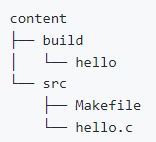
\includegraphics{directory_spdxexample}
	\caption[C Project Directory Structure]{C Project Directory Structure \source{\cite{SPDXExamples}}}
	\label{fig:C Project}
\end{figure}

\noindent
Listing \ref{lst:SPDX Document} shows a corresponding \textit{SPDX Document}. Some tag:value pairs which are less relevant for the overall understanding are deliberately omitted to contain the length of the example.\\ 

\noindent
\begin{lstlisting}[basicstyle=\tiny, caption=SPDX Document, captionpos=b, label=lst:SPDX Document]
SPDXVersion: SPDX-2.2
DataLicense: CC0-1.0
SPDXID: SPDXRef-DOCUMENT
DocumentName: hello
DocumentNamespace: https://swinslow.net/spdx-examples/example1/hello-v3
Creator: Person: Steve Winslow (steve@swinslow.net)
Created: 2021-08-26T01:46:00Z

##### Package: hello
PackageName: hello
SPDXID: SPDXRef-Package-hello
PackageDownloadLocation: git+https://github.com/swinslow/spdx-examples.git#example1/content
PackageLicenseConcluded: GPL-3.0-or-later
PackageLicenseInfoFromFiles: GPL-3.0-or-later
PackageLicenseDeclared: GPL-3.0-or-later
PackageCopyrightText: NOASSERTION

FileName: /build/hello
SPDXID: SPDXRef-hello-binary
FileType: BINARY
LicenseConcluded: GPL-3.0-or-later
LicenseInfoInFile: NOASSERTION
FileCopyrightText: NOASSERTION

FileName: /src/Makefile
SPDXID: SPDXRef-Makefile
FileType: SOURCE
LicenseConcluded: GPL-3.0-or-later
LicenseInfoInFile: GPL-3.0-or-later
FileCopyrightText: NOASSERTION

FileName: /src/hello.c
SPDXID: SPDXRef-hello-src
FileType: SOURCE
LicenseConcluded: GPL-3.0-or-later
LicenseInfoInFile: GPL-3.0-or-later
FileCopyrightText: Copyright Contributors to the spdx-examples project.

Relationship: SPDXRef-hello-binary GENERATED_FROM SPDXRef-hello-src
Relationship: SPDXRef-hello-binary GENERATED_FROM SPDXRef-Makefile
Relationship: SPDXRef-Makefile BUILD_TOOL_OF SPDXRef-Package-hello
\end{lstlisting}

\noindent
Most of the tag:value pairs are self-explanatory, but some might require some explanation. The \textit{Concluded License} is the license the SPDX file creator has concluded as the governing license of a package or a file. \textit{License Information from Files} contains a list of all licenses found in a package and the \textit{Declared License} is the license declared by the authors of the package \cite{SPDXSpec}. Additionally, listing \ref{lst:SPDX Document} illustrates how the concept of relationships may be used.\par
It also worth mentioning that the concept of \textit{Packages} in SPDX as a set of associated files is really rather loose. Thus, describing the project in figure \ref{fig:C Project} as two separate packages, one for source and one for binary, optionally in the same or also in two separate \textit{SPDX Documents} would be completely conform with the specification as well.\par
Since SPDX has been around for so long and is an accepted ISO standard, there exists a lot of useful tooling. It is therefore quite easy to automate tasks like producing, consuming, transforming and validating \textit{SPDX Documents} \cite{SPDXWebsite}.\\

\noindent
While SPDX is a really good standard to describe licensing and copyright information about packages, it has some flaws when being viewed as a standalone SBOM standard. A main point of criticism is associated to how the SPDX specification handles the mapping to other data sources. Through \textit{SPDX External References} it allows a \textit{Package} to reference an external source of information believed to be relevant to the \textit{Package}. This allows one \textit{Package} to have multiple CPEs or package URLs if these references are believed to be relevant. This provides a lot of flexibility, but also means that SPDX does not necessarily uniquely identify each \textit{Package} in the context of other data sources.\\
 
\noindent
\textbf{CycloneDX:}\\
-Further requirements for SBOMs
-Integrate into build system because of the information from package managers
-Ideally incorporate all the ways of creating SBOMs and merge the information somehow

\noindent
\textbf{Software Identification (SWID) tags:}\\

\noindent
\textbf{Open Component Model (OCM):}\\

\subsection{Creation}


\todo{Add a section about supply chain attacks to stress the necessity of SBOMS?}

\section{Vulnerabilities}
\section{OSS Licensing}
\section{Context at SAP Gardener}
Builds, Repositories, Gardener Servicelet Pattern (Session mit Uwe)
\subsection{SAP Gardener}
\subsection{SAP Gardener Deployment Scenario}
\section{Integration into the Application Lifecycle}